\chapter{Dalsza ścieżka rozwoju projektu}
\label{cha:dalsze}
Niniejszy rozdział opisuje sugestie autorów oraz już zaplanowane działania dotyczące dalszego rozwoju projektu \gls*{ggss}, takie jak migracja do nowych standardów języka, zwiększenie jakości kodu czy rozszerzenie projektu o~nowe interfejsy graficzne.

\section{Wprowadzenie zautomatyzowanego systemu testowania projektu}
Przygotowana przez autorów infrastruktura CI/CD pozwala na łatwe wprowadzenie do projektu dużej liczby zautomatyzowanych testów. Testy te powinny dotyczyć zarówno potencjalnych nowych komponentów projektu, jak i~już istniejących, które podlegać będą modyfikacji. Takie działanie pozwala zwiększyć niezawodność tworzonego oprogramowania. Autorzy planują prowadzić dalsze prace z~wykorzystaniem praktyki \textbf{Test Driven Development (TDD)} zakładającej tworzenie testów równolegle z~oprogramowaniem. Stosujący podejście TDD programista najpierw przygotowuje odpowiedni test, a~następnie implementuje funkcjonalność, którą ten test sprawdza. Po wykonaniu tej czynności przechodzi do poprawy jakości już istniejącego kodu, a~następnie powtarza cały cykl. Prawdopodobnie do projektu wprowadzone zostanie również narzędzie \textbf{Coverity} pozwalające na przeprowadzenie statycznej analizy kodu.

\section{Poprawa jakości kodu napisanego w~języku C++}
W swojej obecnej postaci projekt napisany jest w~języku C++ z~elementami standardu C++11. Planowana jest pełna migracja kodu do standardu C++11 lub, jeśli będzie to możliwe (rozwiązany zostanie problem ograniczeń związanych z~infrastrukturą projektu), do standardu C++14 lub C++17. Migracja do nowego standardu oznaczała będzie również wyeliminowanie pewnych zewnętrznych zależności, które dostarczają funkcjonalności będących częścią nowych standardów języka. Dotyczy to przede wszystkim niektórych komponentów biblioteki Boost. Poza zmianami pozwalającymi na modernizację kodu planowane jest również ujednolicenie jego struktury oraz wprowadzenie konwencji dotyczących m.in. nazewnictwa zmiennych czy funkcji. Do tej pory autorom udało się wprowadzić tego typu zmiany w~systemie budowania projektu. 

\section{Automatyzacja procesu publikowania produktu}
Planowany jest dalszy rozwój przygotowanej przez autorów infrastruktury CI/CD. Poza wspomnianymi już wcześniej zautomatyzowanymi testami oprogramowania, wprowadzone może również zostać automatyczne wersjonowanie wydań projektu. Przydatne może się również okazać przygotowanie skryptu aktualizującego zdalne repozytoria projektu po wprowadzeniu zmian w~kilku submodułach. Wymaga to wykonywania operacji \lstinline{git add}, \lstinline{git commit} oraz \lstinline{git push} dla każdego komponentu zależnego od zmodyfikowanych submodułów i~tak dalej aż do komponentu stanowiącego korzeń projektu. Wykonywanie tej czynności manualnie jest niewydajne, stąd też potrzeba przygotowania skryptu automatyzującego tą czynność.


\section{Migracja do języka Python 3}
Znaczna część skryptów w~projekcie \gls*{ggss} napisana została kilka lat temu w~języku Python 2. Z~uwagi na zapowiedziane zakończenie oficjalnego wsparcia dla tej wersji języka sugerowane jest przepisanie skryptów z~użyciem Pythona 3. Migracja dotyczyć może również niektórych skryptów napisanych w~języku \gls*{bash}. 

\section{Przygotowanie dodatkowych interfejsów graficznych}
Od początku pracy autorów nad projektem \gls*{ggss} planowane było rozszerzenie jego funkcjonalności o~nowe interfejsy graficzne pozwalające na wygodne przeglądanie gromadzonych danych. Istnieje wiele możliwych sposobów implementacji takich interfejsów. Jednym z~nich jest zastosowanie popularnego \textbf{framework'u Qt}, przeznaczonego do pracy z~językiem C++. 


\chapter{Podsumowanie}
\label{cha:summary}
Niniejszy rozdział stanowi podsumowanie prac przeprowadzonych przez autorów nad projektem \gls*{ggss}. Zaprezentowane zostaną statystyki związane z~projektem oraz wkładem autorów w~jego rozwój, jak również zbiór wniosków, wyciągniętych przez autorów podczas prac nad systemem. 

Zadaniem autorów było przeprowadzenie rozbudowy i~aktualizacji oprogramowania Systemu Stabilizacji Wzmocnienia Gazowego detektora ATLAS \gls*{trt}. Przeprowadzona została zmiana architektury projektu oraz systemu budującego, wprowadzone zostały nowe rozwiązania, takie jak infrastruktura CI/CD oraz system kontroli wersji \gls*{git}. Pojawiło się wiele udoskonaleń względem poprzedniego rozwiązania, m.in. w~logice działania pakietu \gls*{rpm}.
Zadaniem autorów przyjęta podczas prac nad projektem strategia polegająca na dogłębnym analizowaniu postawionych przed nimi zadań była opłacalna. Poświęcenie czasu na dokładne przemyślenie rozwiązania pozwoliło autorom na znaczne przyspieszenie prac w~fazie realizacji. Pozytywnym aspektem przeprowadzonych prac był również ich zespołowy charakter - pozwoliło to autorom na szybszą eliminację napotkanych problemów oraz dawało możliwość dzielenia się swoją wiedzą. Wkład obu autorów w~projekt jest porównywalny, co obrazuje tabela \ref{table:stats2}. Wskazuje to na dobry przebieg współpracy między autorami. Praca nad systemem będącym częścią międzynarodowego projektu pozwoliła autorom również na zdobycie cennego, unikalnego doświadczenia.
Zdaniem autorów wszystkie postawione przed nimi zadania zostały realizowane. Prace nad projektem będą kontynuowane w~dalszym toku studiów podejmowanych przed autorów.


\begin{table*}[htbp]
\centering
\caption{Ilość linii w~plikach projektu}
\label{table:stats1}
\begin{tabular}{@{}lr@{}}
\toprule
Typ plików & 
Ilość linii zawarta we wszystkich plikach danego typu \\

\midrule

C/C++               & 18 011 \\
CMake               & 1 412 \\
Python              & 602 \\
Markdown            & 557 \\
.gitlab-ci.yml      & 430 \\
Shell/Bash          & 336 \\
Dockerfile          & 56 \\
\textbf{RAZEM}      & 21 404 \\

\bottomrule
\end{tabular}
\end{table*}


\begin{table*}[htbp]
\centering
\caption{Statystyki wkładu autorów w~projekt uzyskane za pomocą portalu GitLab}
\label{table:stats2}
\begin{tabularx}{\textwidth}{@{}XXXX@{}}
\toprule
Osoba &
Ilość commit'ów &
\begin{tabular}[x]{@{}l@{}}Ilość wykonanych \\merge request'ów \end{tabular}& 
\begin{tabular}[x]{@{}l@{}}Ilość zamkniętych \\issue \end{tabular}\\

\midrule

Jarosław Cierpich & 150 & 11 & 14 \\
Arkadiusz Kasprzak & 212 & 6 & 12 \\

\bottomrule
\end{tabularx}
\end{table*}


\appendix
\chapter{Dodatki/Appendixes}
\label{cha:app}
Niniejsza część pracy zawiera trzy dodatki dotyczące procesu przygotowywania maszyny wirtualnej do pracy jako tzw. \textit{runner} z~narzędziem GitLab CI/CD, procesu dodawania nowych modułów do projektu \gls*{ggss} oraz struktury projektu przed i~po wprowadzeniu przez autorów zmian. Dwa z~dodatków przygotowane zostały w~języku angielskim - powodem tego jest międzynarodowy charakter zespołu pracującego nad detektorem \gls*{trt} oraz fakt, że dodatki te stanowią część dokumentacji znajdującej się w~repozytoriach projektu.

This part of the dissertation contains three appendixes that cover following topics: preparing the virtual machine to work as a~GitLab CI/CD runner, adding new modules to the \gls*{ggss} project using templates created by authors and comparing the project structure before and after changes. Two of the appendixes were written in English - that's due to the international nature of the \gls*{trt} community as well as the fact that those appendixes are a~part of documentation that can be found in project's repositories. 

\section{Porównanie początkowej i~obecnej struktury projektu oraz kodu źródłowego}

Niniejszy dodatek przedstawia porównanie początkowej oraz końcowej struktury projektu \gls*{ggss}. Listing \ref{lst:compareStructure} przedstawia porównanie katalogów na poziomie całego projektu, gdzie tymi samymi kolorami oznaczone zostały odpowiadające sobie komponenty. Kolorem czarnym oznaczone zostały katalogi nieposiadające odpowiedników.

Listing \ref{lst:newLibStructure} przedstawia porównanie struktury biblioteki \textbf{ggss-lib} po wprowadzonych zmianach oraz przed nimi. Takie zmiany zostały wprowadzone w~każdej z~bibliotek wchodzących w~skład projektu \gls*{ggss}.


Rysunki \ref{fig:addExternC} i~\ref{fig:removeExternC} przedstawiają jedyne zmiany wprowadzone bezpośrednio w~kodzie źródłowym aplikacji.

\newpage



\definecolor{plum(traditional)}{rgb}{0.56, 0.27, 0.52}
\definecolor{amber(sae/ece)}{rgb}{1.0, 0.49, 0.0}
\definecolor{cadmiumgreen}{rgb}{0.0, 0.42, 0.24}
\definecolor{capri}{rgb}{0.0, 0.75, 1.0}
\definecolor{sinopia}{rgb}{0.8, 0.25, 0.04}
\definecolor{salmon}{rgb}{0.9, 0.55, 0.51}
\definecolor{fyellow}{rgb}{0.44, 0.65, 0.82}

\def\redcolor{\color{red}}
\def\blackcolor{\color{black}}
\def\greencolor{\color{green}}
\def\purplecolor{\color{plum(traditional)}}
\def\bluecolor{\color{blue}}
\def\ambercolor{\color{amber(sae/ece)}}
\def\darkgreencolor{\color{cadmiumgreen}}
\def\capricolor{\color{capri}}
\def\magentacolor{\color{magenta}}
\def\sinopiacolor{\color{sinopia}}
\def\yellowcolor{\color{salmon}}
\def\fyellowcolor{\color{fyellow}}

\begin{multicols*}{2}[\captionof{lstlisting}{Porównanie aktualnej i pierwotnej struktury katalogów. Odpowiadające sobie elementy zostały oznaczone jednym kolorem.}]
\begin{lstlisting}[language=Cmd, title={(a) Aktualna struktura katalogów}, escapechar=@, label={lst:compareStructure}]
.
|-- @\aftergroup\redcolor@ggss-dim-cs@\aftergroup\blackcolor@
|   |-- @\aftergroup\greencolor@external-dim-lib@\aftergroup\blackcolor@
|   `-- @\aftergroup\greencolor@ggss-misc@\aftergroup\blackcolor@
|-- @\aftergroup\purplecolor@ggss-driver@\aftergroup\blackcolor@
|   |-- @\aftergroup\greencolor@external-n957-lib@\aftergroup\blackcolor@
|   |-- @\aftergroup\greencolor@ggss-misc@\aftergroup\blackcolor@
|   `-- @\aftergroup\purplecolor@n957@\aftergroup\blackcolor@
|-- @\aftergroup\fyellowcolor@ggss-oper@\aftergroup\blackcolor@
|   |-- @\aftergroup\fyellowcolor@localdisk-scripts@\aftergroup\blackcolor@
|   `-- @\aftergroup\fyellowcolor@opt-scripts@\aftergroup\blackcolor@
|-- @\aftergroup\magentacolor@ggss-runner@\aftergroup\blackcolor@
|   `-- @\aftergroup\capricolor@ggss-lib@\aftergroup\blackcolor@
|       |-- @\aftergroup\greencolor@external-dim-lib@\aftergroup\blackcolor@
|       |-- @\aftergroup\ambercolor@ggss-hardware-libs@\aftergroup\blackcolor@
|       |   |-- @\aftergroup\ambercolor@caenhv-lib@\aftergroup\blackcolor@
|       |   |-- @\aftergroup\ambercolor@caenn1470-lib@\aftergroup\blackcolor@
|       |   |-- @\aftergroup\greencolor@external-n957-lib@\aftergroup\blackcolor@
|       |   |-- @\aftergroup\bluecolor@ggss-util-libs@\aftergroup\blackcolor@
|       |   |   |-- @\aftergroup\greencolor@ggss-misc@\aftergroup\blackcolor@
|       |   |   |-- @\aftergroup\bluecolor@handle-lib@\aftergroup\blackcolor@
|       |   |   |-- @\aftergroup\bluecolor@log-lib@\aftergroup\blackcolor@
|       |   |   |-- @\aftergroup\bluecolor@thread-lib@\aftergroup\blackcolor@
|       |   |   `-- @\aftergroup\bluecolor@utils-lib@\aftergroup\blackcolor@
|       |   |-- @\aftergroup\ambercolor@mca-lib@\aftergroup\blackcolor@
|       |   |-- @\aftergroup\ambercolor@ortecmcb-lib@\aftergroup\blackcolor@
|       |   `-- @\aftergroup\ambercolor@usbrm-lib@\aftergroup\blackcolor@
|       `-- @\aftergroup\darkgreencolor@ggss-software-libs@\aftergroup\blackcolor@
|           |-- @\aftergroup\darkgreencolor@daemon-lib@\aftergroup\blackcolor@
|           |-- @\aftergroup\darkgreencolor@fifo-lib@\aftergroup\blackcolor@
|           |-- @\aftergroup\darkgreencolor@fit-lib@\aftergroup\blackcolor@
|           |-- @\aftergroup\bluecolor@ggss-util-libs@\aftergroup\blackcolor@
|           `-- @\aftergroup\darkgreencolor@xml-lib@\aftergroup\blackcolor@
|-- @\aftergroup\sinopiacolor@ggss-spector@\aftergroup\blackcolor@
`-- @\aftergroup\yellowcolor@mca-n957@\aftergroup\blackcolor@
    `-- @\aftergroup\ambercolor@ggss-hardware-libs@\aftergroup\blackcolor@
\end{lstlisting}
\vfill\null
\columnbreak
\begin{lstlisting}[language=Cmd, title={(b) Pierwotna struktura katalogów} ,escapechar=@]
.
|-- caen_n957
|   |-- @\aftergroup\yellowcolor@_mca@\aftergroup\blackcolor@
|   |-- @\aftergroup\ambercolor@mcaLib@\aftergroup\blackcolor@
|   `-- @\aftergroup\ambercolor@OrtecMcbLib@\aftergroup\blackcolor@
|-- ggss-bin
|   |-- @\aftergroup\ambercolor@CaenHVLib@\aftergroup\blackcolor@
|   |-- @\aftergroup\ambercolor@CaenN1470Lib@\aftergroup\blackcolor@
|   |-- @\aftergroup\darkgreencolor@daemonLib@\aftergroup\blackcolor@
|   |-- @\aftergroup\redcolor@_dimCS@\aftergroup\blackcolor@
|   |-- @\aftergroup\darkgreencolor@fifoLib@\aftergroup\blackcolor@
|   |-- @\aftergroup\darkgreencolor@FitLib@\aftergroup\blackcolor@
|   |-- @\aftergroup\magentacolor@_ggss@\aftergroup\blackcolor@
|   |-- @\aftergroup\capricolor@ggssLib@\aftergroup\blackcolor@
|   |-- @\aftergroup\sinopiacolor@_ggsspector@\aftergroup\blackcolor@
|   |-- @\aftergroup\bluecolor@handleLib@\aftergroup\blackcolor@
|   |-- @\aftergroup\greencolor@include@\aftergroup\blackcolor@
|   |-- @\aftergroup\greencolor@lib@\aftergroup\blackcolor@
|   |-- @\aftergroup\bluecolor@logLib@\aftergroup\blackcolor@
|   |-- @\aftergroup\ambercolor@mcaLib@\aftergroup\blackcolor@
|   |-- misc
|   |   |-- config
|   |   |-- n957_old
|   |   `-- python
|   |-- @\aftergroup\ambercolor@OrtecMcbLib@\aftergroup\blackcolor@
|   |-- @\aftergroup\fyellowcolor@scripts@\aftergroup\blackcolor@
|   |-- @\aftergroup\bluecolor@ThreadLib@\aftergroup\blackcolor@
|   |-- @\aftergroup\ambercolor@usbrmLib@\aftergroup\blackcolor@
|   |-- @\aftergroup\bluecolor@utilsLib@\aftergroup\blackcolor@
|   `-- @\aftergroup\darkgreencolor@xmlLib@\aftergroup\blackcolor@
`-- @\aftergroup\purplecolor@ggss-driver@\aftergroup\blackcolor@
    `-- @\aftergroup\purplecolor@n957@\aftergroup\blackcolor@
\end{lstlisting}

\end{multicols*}

\newpage

\begin{multicols*}{2}[\captionof{lstlisting}{Porównanie aktualnej i pierwotnej struktury biblioteki \textbf{ggss-lib}. Odpowiadające sobie elementy zostały oznaczone jednym kolorem.}]
\begin{lstlisting}[title={(a) Nowa struktura biblioteki \textbf{ggss-lib}}, label={lst:newLibStructure}, escapechar=@]
.
|-- ggss-software-libs
|-- ggss-hardware-libs
|-- external-dim-lib
|-- @\aftergroup\darkgreencolor@CMakeLists.txt@\aftergroup\blackcolor@
|-- include
|   `-- ggssLib
|       |-- @\aftergroup\bluecolor@ChannelDataForDim.h@\aftergroup\blackcolor@
|       |-- @\aftergroup\bluecolor@ChannelData.h@\aftergroup\blackcolor@
|       |-- @\aftergroup\bluecolor@Channel.h@\aftergroup\blackcolor@
|       |-- @\aftergroup\bluecolor@ChannelParamsForDim.h@\aftergroup\blackcolor@
|       |-- @\aftergroup\bluecolor@DimGgssEventListener.h@\aftergroup\blackcolor@
|       |-- @\aftergroup\bluecolor@GgssDataForDim.h@\aftergroup\blackcolor@
|       |-- @\aftergroup\bluecolor@GgssEventListener.h@\aftergroup\blackcolor@
|       |-- @\aftergroup\bluecolor@GgssEventLoopRunner.h@\aftergroup\blackcolor@
|       |-- @\aftergroup\bluecolor@ggssExceptions.h@\aftergroup\blackcolor@
|       |-- @\aftergroup\bluecolor@ggss.h@\aftergroup\blackcolor@
|       |-- @\aftergroup\bluecolor@GgssParamsForDim.h@\aftergroup\blackcolor@
|       `-- @\aftergroup\bluecolor@ggssParams.h@\aftergroup\blackcolor@
|-- README.md
`-- src
    |-- @\aftergroup\redcolor@Channel.cpp@\aftergroup\blackcolor@
    |-- @\aftergroup\redcolor@ChannelData.cpp@\aftergroup\blackcolor@
    |-- @\aftergroup\redcolor@ChannelDataForDim.cpp@\aftergroup\blackcolor@
    |-- @\aftergroup\redcolor@ChannelParamsForDim.cpp@\aftergroup\blackcolor@
    |-- @\aftergroup\redcolor@DimGgssEventListener.cpp@\aftergroup\blackcolor@
    |-- @\aftergroup\redcolor@ggss.cpp@\aftergroup\blackcolor@
    |-- @\aftergroup\redcolor@GgssDataForDim.cpp@\aftergroup\blackcolor@
    |-- @\aftergroup\redcolor@GgssEventLoopRunner.cpp@\aftergroup\blackcolor@
    |-- @\aftergroup\redcolor@ggssParams.cpp@\aftergroup\blackcolor@
    `-- @\aftergroup\redcolor@GgssParamsForDim.cpp@\aftergroup\blackcolor@

\end{lstlisting}

\vfill\null
\columnbreak

\begin{lstlisting}[title={(b) Pierwotna struktura biblioteki \textbf{ggss-lib}}, label={lst:oldLibStructure}, escapechar=@]
ggssLib/
|-- @\aftergroup\redcolor@Channel.cpp@\aftergroup\blackcolor@
|-- @\aftergroup\redcolor@ChannelData.cpp@\aftergroup\blackcolor@
|-- @\aftergroup\redcolor@ChannelDataForDim.cpp@\aftergroup\blackcolor@
|-- @\aftergroup\bluecolor@ChannelDataForDim.h@\aftergroup\blackcolor@
|-- @\aftergroup\bluecolor@ChannelData.h@\aftergroup\blackcolor@
|-- @\aftergroup\bluecolor@Channel.h@\aftergroup\blackcolor@
|-- @\aftergroup\redcolor@ChannelParamsForDim.cpp@\aftergroup\blackcolor@
|-- @\aftergroup\bluecolor@ChannelParamsForDim.h@\aftergroup\blackcolor@
|-- @\aftergroup\darkgreencolor@CMakeLists.txt@\aftergroup\blackcolor@
|-- @\aftergroup\redcolor@DimGgssEventListener.cpp@\aftergroup\blackcolor@
|-- @\aftergroup\bluecolor@DimGgssEventListener.h@\aftergroup\blackcolor@
|-- @\aftergroup\redcolor@ggss.cpp@\aftergroup\blackcolor@
|-- @\aftergroup\redcolor@GgssDataForDim.cpp@\aftergroup\blackcolor@
|-- @\aftergroup\bluecolor@GgssDataForDim.h@\aftergroup\blackcolor@
|-- @\aftergroup\bluecolor@GgssEventListener.h@\aftergroup\blackcolor@
|-- @\aftergroup\redcolor@GgssEventLoopRunner.cpp@\aftergroup\blackcolor@
|-- @\aftergroup\bluecolor@GgssEventLoopRunner.h@\aftergroup\blackcolor@
|-- @\aftergroup\bluecolor@ggssExceptions.h@\aftergroup\blackcolor@
|-- @\aftergroup\bluecolor@ggss.h@\aftergroup\blackcolor@
|-- @\aftergroup\redcolor@ggssParams.cpp@\aftergroup\blackcolor@
|-- @\aftergroup\redcolor@GgssParamsForDim.cpp@\aftergroup\blackcolor@
|-- @\aftergroup\bluecolor@GgssParamsForDim.h@\aftergroup\blackcolor@
`-- @\aftergroup\bluecolor@ggssParams.h@\aftergroup\blackcolor@
\end{lstlisting}

\end{multicols*}

\newpage

\begin{figure}
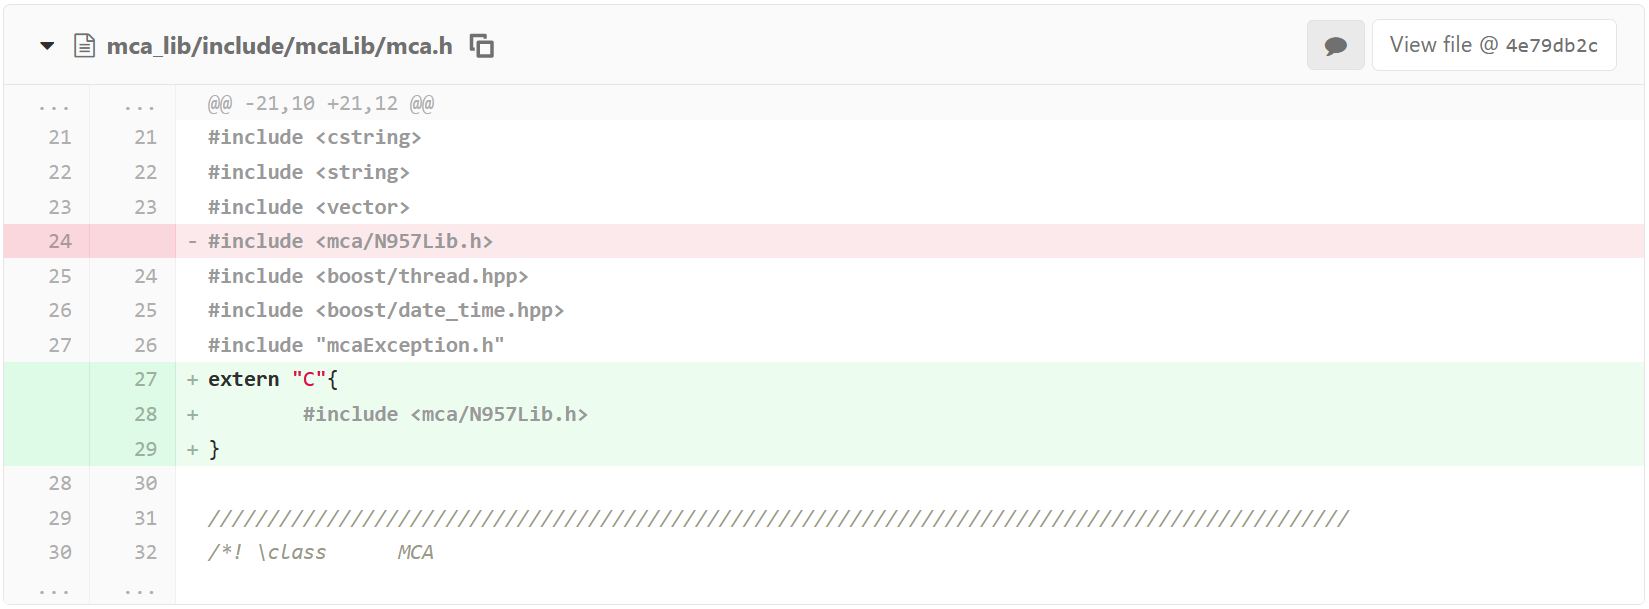
\includegraphics[width=\textwidth]{res/png/addExternC}
\caption{Dodanie konstrukcji \lstinline[language=c++]{extern "C"} w~ramach biblioteki \textbf{mca-lib}}
\label{fig:addExternC}
\end{figure}

\begin{figure}
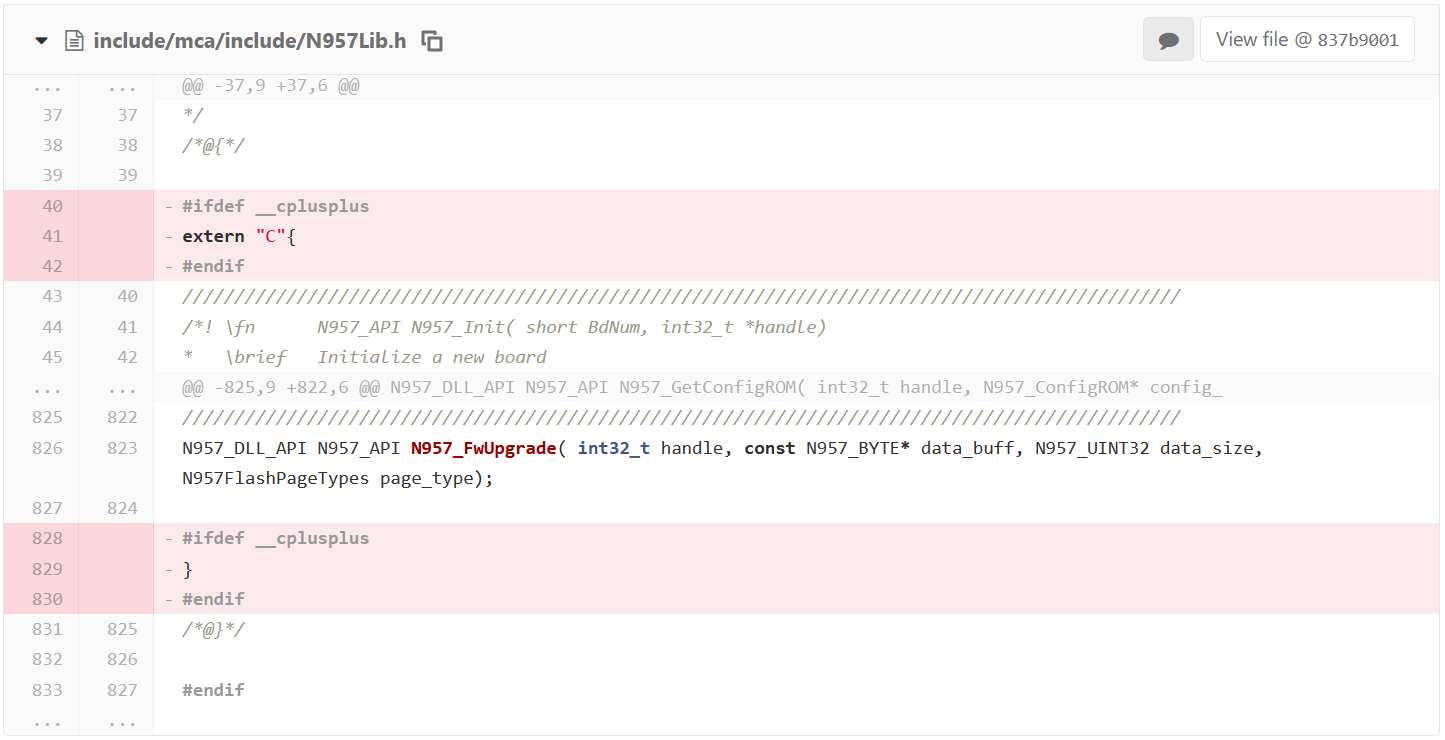
\includegraphics[width=\textwidth]{res/png/removeExternC}
\caption{Usunięcie konstrukcji \lstinline[language=c++]{extern "C"} w~ramach zewnętrznej biblioteki \textbf{CAENN957}}
\label{fig:removeExternC}
\end{figure}

\onecolumn

\includepdfset{pages=-,pagecommand=\thispagestyle{fancy}}
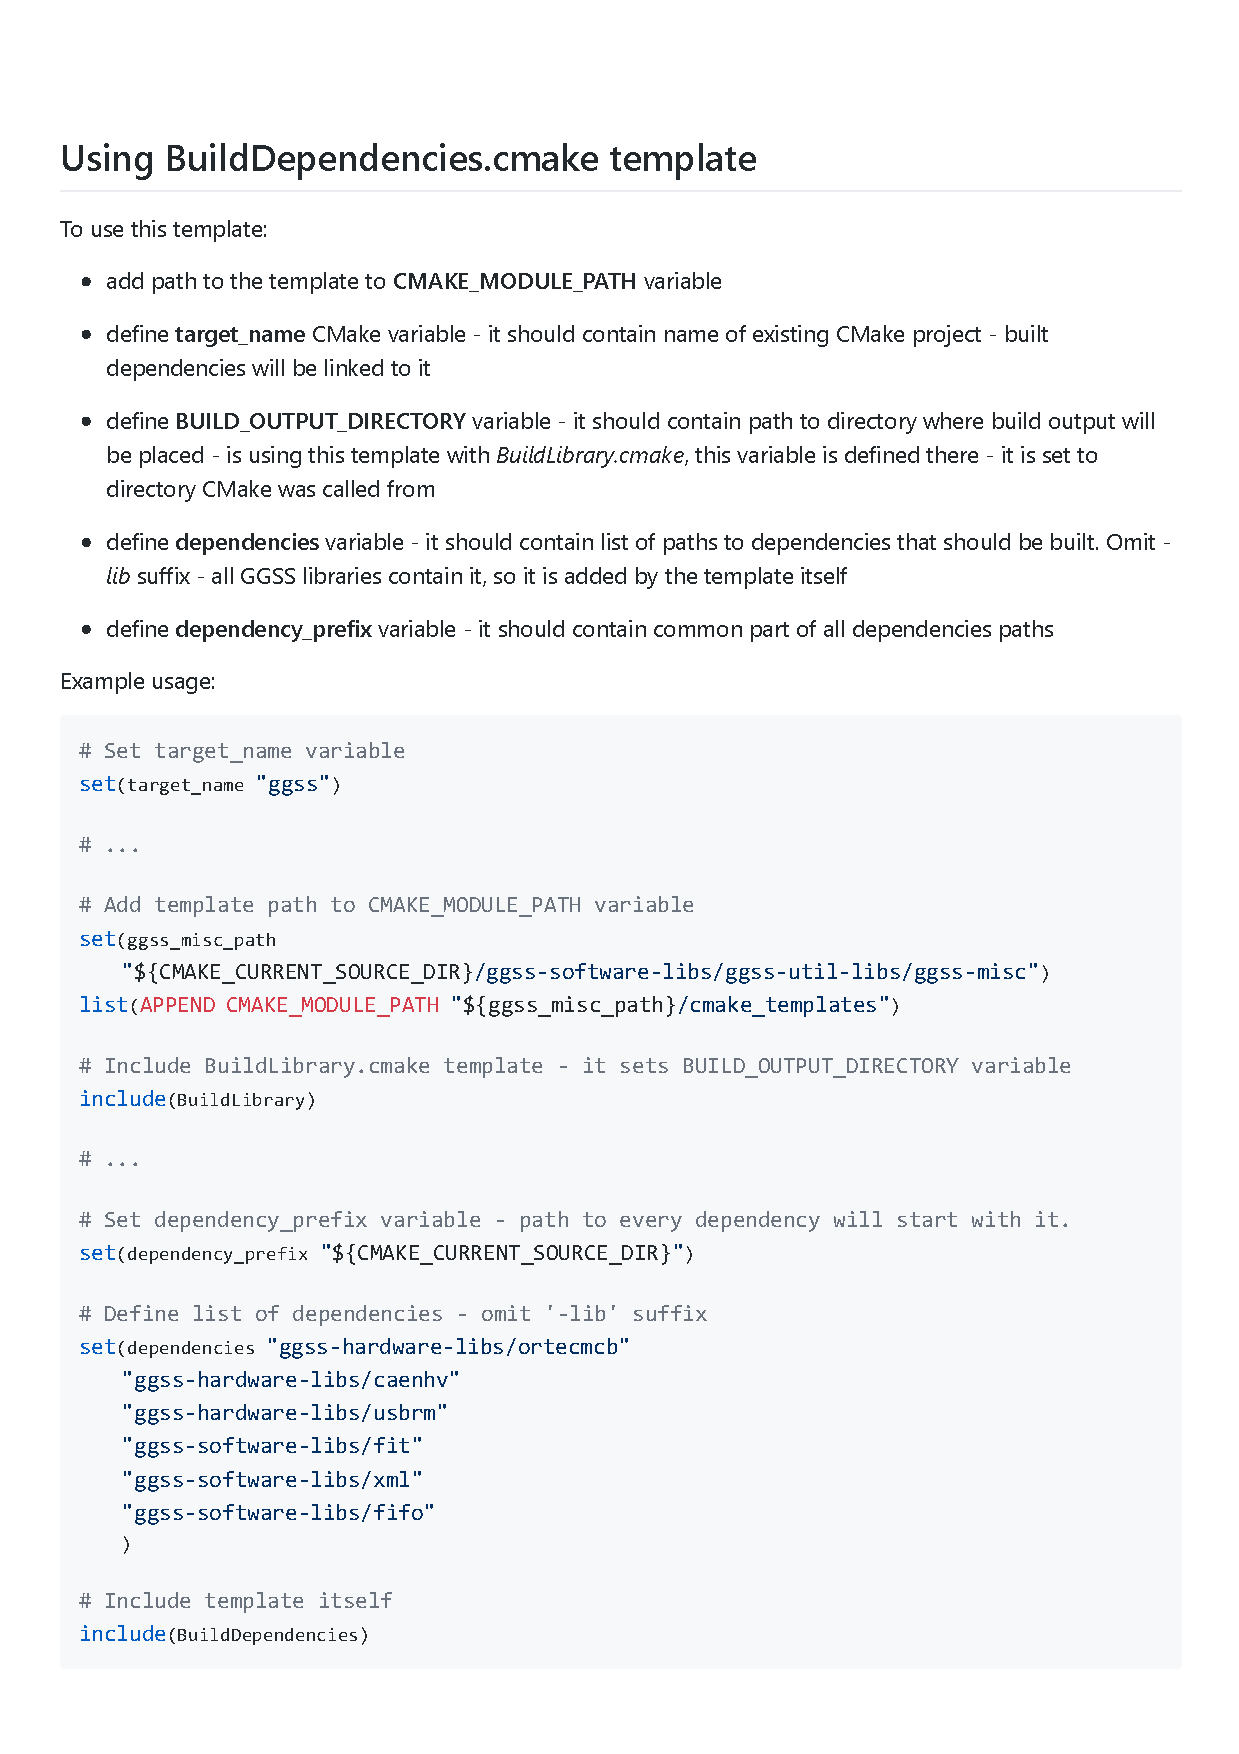
\includepdf[pages=1, scale=0.8,offset= 0.65cm -1.2cm, pagecommand={\section{Adding modules to the project using existing CMake templates\label{appendix:A2}}}]{res/UsingCMakeTemplates.pdf}
\includepdf[pages=2,scale=0.8,offset= 0.65cm 0]{res/UsingCMakeTemplates.pdf}

\newpage

\includepdfset{pages=-,pagecommand=\thispagestyle{fancy}}
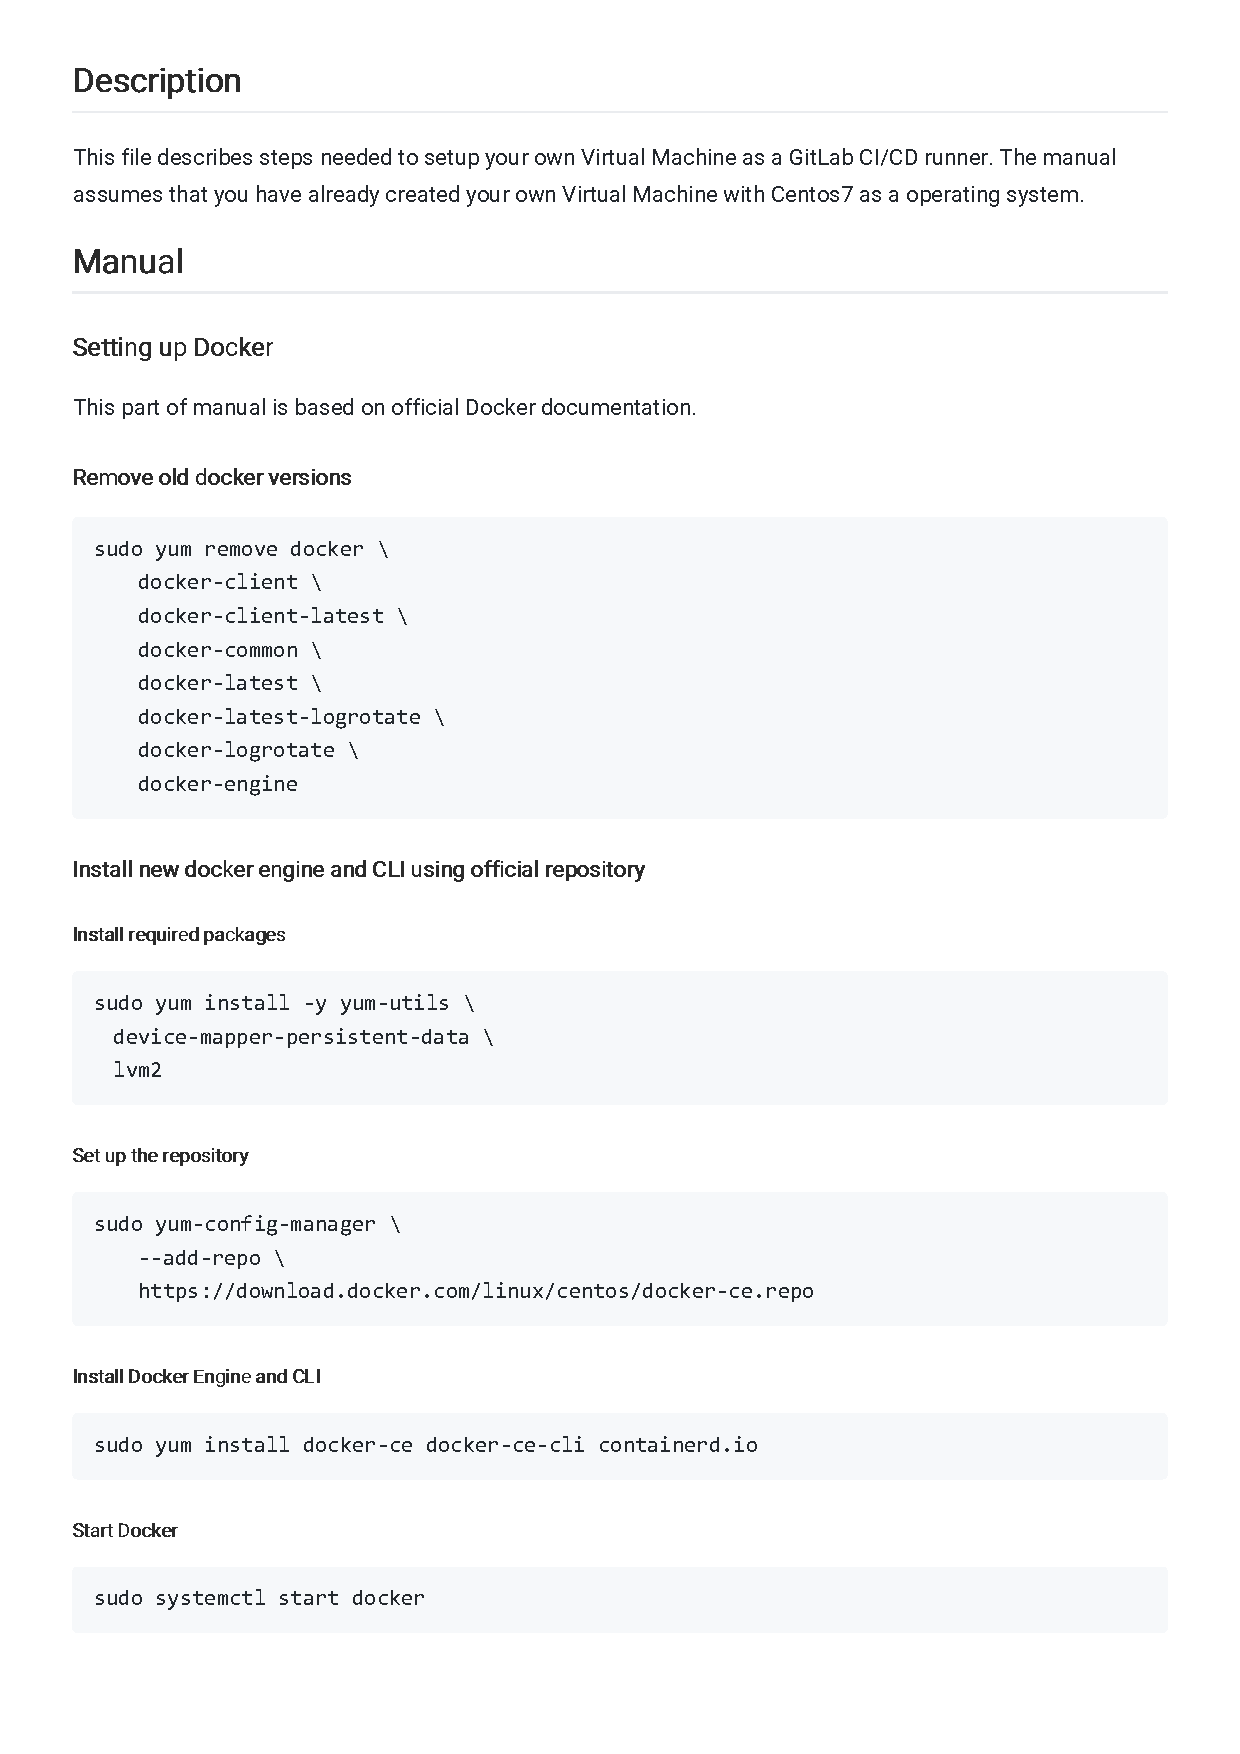
\includepdf[pages=1, scale=0.85,offset= 0.65cm -1cm, pagecommand={\section{Preparing the virtual machine to work as a~runner\label{appendix:A3}}}]{res/howToRunner.pdf}
\includepdf[pages=2,scale=0.85,offset= 0.65cm 0]{res/howToRunner.pdf}
\includepdf[pages=3,scale=0.85,offset= 0.65cm 0]{res/howToRunner.pdf}

Dodatek \ref{appendix:A3} opisuje procedurę dodawania nowej maszyny jako GitLab CI/CD Runner (jednostka odpowiedzialna za wykonywanie zadań w~ramach funkcjonalności GitLab CI/CD). Instrukcja zakłada, że maszyna posiada zainstalowany system operacyjny Linux w~dystrybucji \textbf{Centos7}. Wynikiem wykonania wszystkich czynności powinno być dodanie maszyny do panelu \textit{CI/CD>Runners} dla wybranej grupy, co ukazuje Rysunek \ref{fig:runner}. Instrukcja została napisana w~oparciu o~dokumentację Docker \cite{DockerInstall} oraz dokumentację GitLab \cite{RunnerRegister}.

\begin{figure}
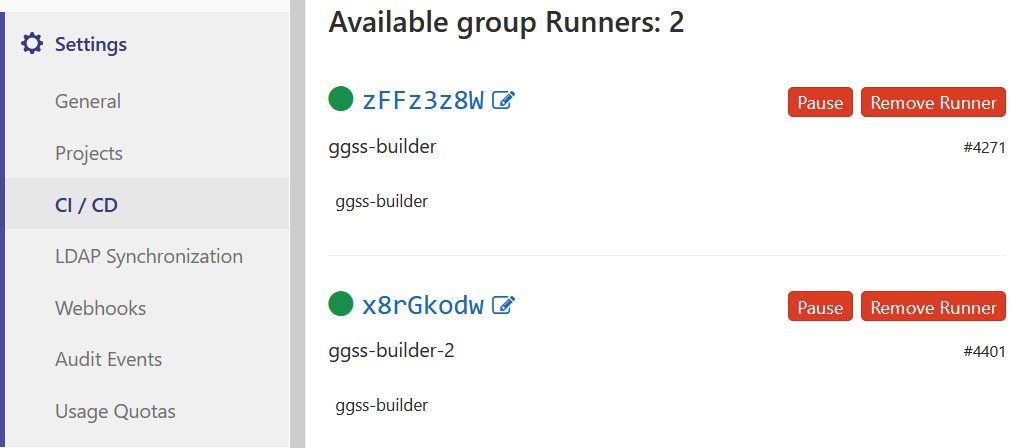
\includegraphics[width=\textwidth]{res/png/runnerAdded}
\caption{Panel przedstawiający dodane GitLab CI/CD Runner w~ramach projektu.}
\label{fig:runner}
\end{figure}
